\chapter{Implementation Approach}
\label{chap:implementation}
\lhead{\emph{Implementation Approach}}

%The key question to be addressed in this chapter is: "How do I plan to achieve what I have outlined in the previous chapter".

%This chapter should comprise around 5000 words and specify your planned implementation approach. Again all sections below are suggestions and will vary significantly from project to project, the key element to be addressed is the core question of the chapter.

\section{Architecture} \label{sec:Arch}
%Describe the architecture of the solution that you have in mind, including:
%\begin{itemize}
%    \item Technologies involved (e.g., frameworks, programming language). 
%    \item The hardware needed to develop the project (and to support at deployment stage)
%\end{itemize}

%Provide a high level view of the system you have in mind, including any package of classes, what is it responsible for and what other packages it communicates to. Provide a high level view of the database (or structure) needed to support the project, including what each table/document is responsible for and the hierarchy among them. You need to be as specific here as you can, why? Because this will aid you in identifying parts of the project you are vague on, this may be fine for some components but cause problems in term 2 for others. If you have hardware element in your project this is also where you provide a high level view of how these elements integrate into the project. So for a project that is cyber-physical you will have both a hardware and software architectural diagram. N.B. This is NOT a full system design but a high level overview of what you can credibly develop. This architecture should be informed by prototyping activity. 

%Some of the implementation focused projects may describe how do you envision tackling the functional requirements of your project via a set of use-cases. DFDs are also helpful here to understand elements of your project that may cause problems. You should describe the role of the different parts of the architecture of the solution, and the interaction among them.

Designing a software architecture is a crucial step of creating software. This will attempt to illuminate any uncertainties that come up with the functionality or implementation. Planning out the architecture before coding often results in a more stable and scalable software. This section will be dedicated to explaining how the project is going to work. The technologies and languages used for this project will be introduced as needed. High level diagrams and class diagrams will accompany the explanation, these diagrams will most likely change during the implementation phase as it would be rather amazing if I got every thing correct here.

The project will be written in C++ as it is a binary compiled language resulting in fast execution of code, this is required as synchronisation takes up a reasonable amount of execution time. C++ has libraries for dealing with networking and threads therefore building an API will be no problem. I also plan on doing a NodeJs module for easy integration with the API using any NodeJS application, this will be done in JavaScript.

\begin{figure}[!h]
  \centering
      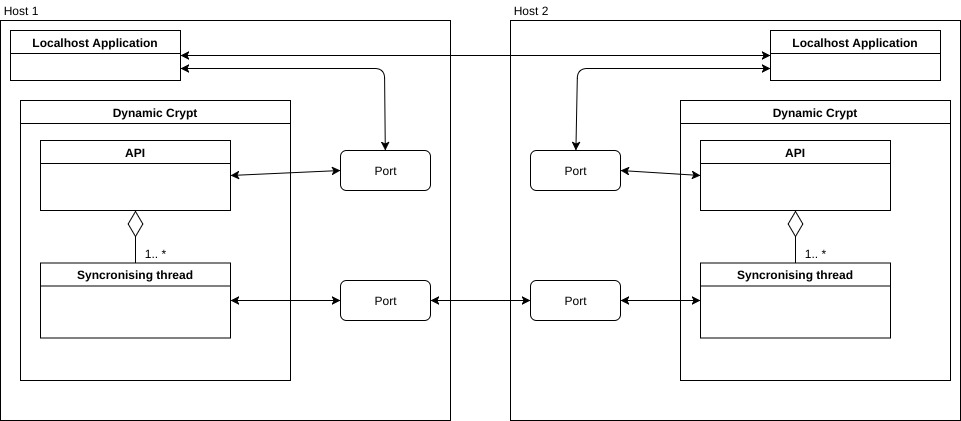
\includegraphics[width=1\textwidth]{Figures/basic-2hosts.jpg}
  \caption[Two hosts using Dynamic Crypt System]{Two hosts using Dynamic Crypt System}
  \label{fig:2hostsbasic}
\end{figure}

\FloatBarrier

The diagram \ref{fig:2hostsbasic} shows a very high level overview of the system in action. There are two hosts in this example. Each host has a localhost Application which is any application that uses the API, it can be a python web application, NodeJS web application, PHP web application etc... 

Each host has a Dynamic Crypt software running which is what this project is about. 

The Dynamic Crypt has two main sort of components if you like. The API which is responsible for communication between applications running on localhost only for security purposes. The localhost applications communicate with the API through a port that will be configured with iptables to only be available for local addressees only so 127.0.0.1 only. 

The Synchronising thread "component" is a single Tree Parity Machine as well as the necessary functionality required for networking and synchronisation between the partner thread of the other host. Each synchronising thread will have its own unique id as well as the partner thread id, IP, port etc.. from the other host in order to be able to send packets directed at the partner thread. This is needed because there will be multiple instances or threads for each host connected to a host. In the host 1 to host 2 example there will most likely be only ten threads synchronising with each other this is to ensure a steady supply of encryption keys, this number of threads for each host may change during the implementation phase. 

How all of this works is going to be similar to the following. 

Host 1: Localhost application establishes a connection with Host 2: Localhost application using standard methods. 

When local Host 1: Localhost application wants to use dynamic encryption to send data to Host 2: Localhost application it contacts the Host 1: Dynamic Crypt API with an init request. 

Host 1: Dynamic Crypt API takes note of Host 1: Localhost application details such as the applications name or port number to distinguish the application from other local host applications as will be demonstrated in a later example. and initialises ten Synchronising threads. The API associates this list of synchronising threads with the application and sends back the details of each thread, the port the threads will use and the IP of Host 1 to Host 1: Localhost application.

Host 1: Localhost application then essentially forwards this information to Host 2: Localhost application which will know that this is an dynamic synchronisation init request and will forward that information to Host 2: Dynamic Crypt API through the Host 2: Dynamic Crypt API port. The Host 2: Dynamic Crypt API will initialise ten Synchronising threads and assigns a partner to them which is essentially the partner id of one of the Host 1: Dynamic Crypt threads.

Host 2: Dynamic Crypt threads will send a request to Host 1: Dynamic Crypt threads. The Thread manager will then forward the info to each thread assigning the partners thread id for Host 1 threads. Now synchronisation between threads will occur how synchronisation occurs is discussed in the research phase but I will provide a diagram shortly.

When a thread is synchronised the API of both hosts will notify the corresponding Localhost application that dynamic synchronisation may occur. The key of the synchronised thread is saved in the API and the thread is forced to desynchronise and begin synchronisation again in order to get a new key. These keys will be added in a queue on both of the hosts API.

The Localhost application can now call the API with an encrypt message request and pass a message to be encrypted. The API uses a key to encrypt a message then the key is discarded from the API, the encrypted message is returned to the Localhost application for ready for sending. 

The message arrives at the other Localhost application. The Localhost application will send a decrypt request to the API with the encrypted message. The API will use the appropriate key to decrypt the message and send it back to the Localhost application. 









\begin{figure}[!h]
  \centering
      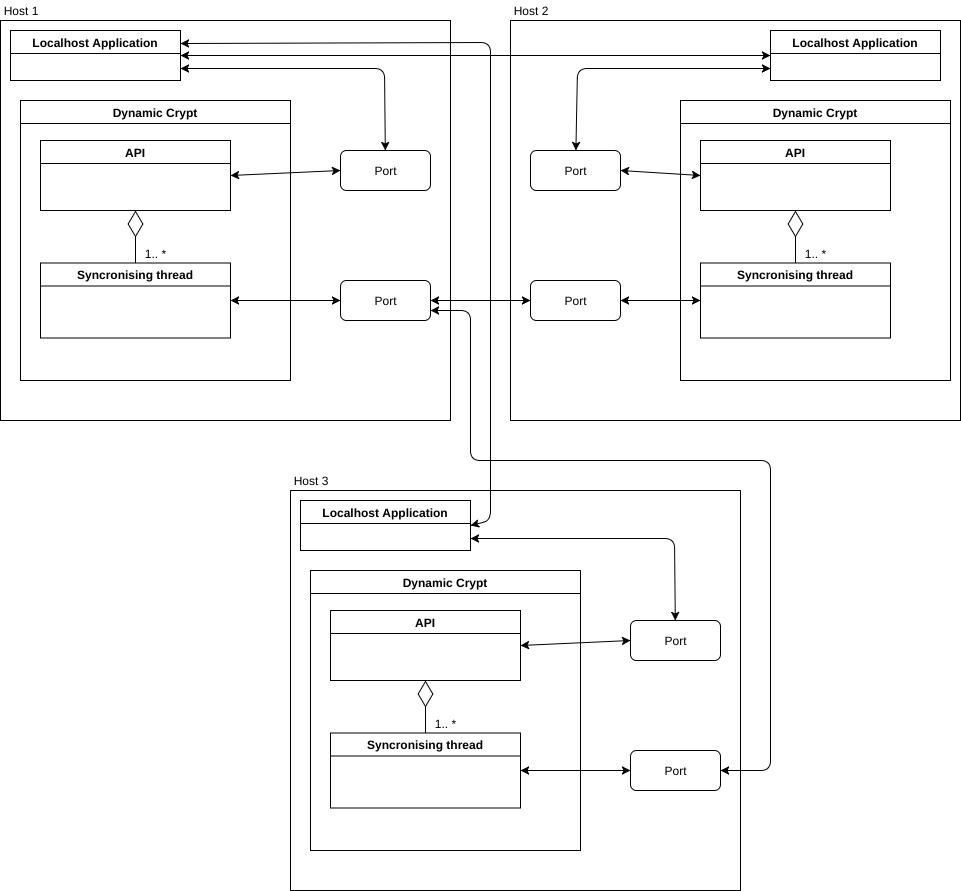
\includegraphics[width=1\textwidth]{Figures/basic-3hosts.jpg}
  \caption[Host one using Dynamic Crypt System with host two and three at the same time]{Host one using Dynamic Crypt System with host two and three at the same time}
  \label{fig:3hostsbasic}
\end{figure}

\FloatBarrier

The diagram \ref{fig:3hostsbasic} demonstrates how dynamic encryption can be implemented when Host 1: Localhost application wishes to send dynamically encrypted information between Host 2 and Host 3 simultaneously. Because Host 1 is attempting to use dynamic encryption to communicate between Host 2 and Host 3 only this means that Host 2 and Host 3 are not aware of each other as there is no need for them to communicate.

This works in quite a similar fashion as with only two hosts but now there are three.

Host 1: Localhost application establishes a connection with Host 2: Localhost application and Host 1: Localhost application establishes a connection with Host 3: Localhost application using standard methods more than likely this will happen one after the other as extra data might be required from Host 3, however there is not going to cause any problems doing it at the same time. 

Host 1: Localhost contacts the Host 1: Dynamic Crypt API with an init request twice one for Host 2 and Host 3. In the init request Host 1: Localhost application also provides any name for Host 2 and Host 3 to distinguish quickly between the two later on.

Host 1: Dynamic Crypt API takes note of Host 1: Localhost application details such as the applications name or port number and the name given to Host 2 and Host 3, and initialises ten Synchronising threads for Host 2 and another ten Synchronising threads for host 3. The API associates this list of synchronising threads with the application and sends back the details of each thread, the port the threads will use, the IP of Host 1 and lastly the name given to Host 2 and Host 3 to Host 1: Localhost application. These details are sent back for Host 2 and Host 3 separately to allow for easy growth since Host 1 might want to dynamically encrypt information and send it to Host 3 much later than Host 2.

Host 1: Localhost application then essentially forwards this information to Host 2: Localhost application and Host 3: Localhost application these will know that this is an dynamic synchronisation init request and will forward that information to Host 2: Dynamic Crypt API through the Host 2: Dynamic Crypt API port and Host 3: Dynamic Crypt API through the Host 3: Dynamic Crypt API port. The Host 2: Dynamic Crypt API and Host 3: Dynamic Crypt API will each initialise ten Synchronising threads and assign a partner to them which is essentially the partner id of one of the Host 1: Dynamic Crypt threads.

Host 2: Dynamic Crypt threads will send a request to Host 1: Dynamic Crypt threads followed by another request from Host 3: Dynamic Crypt threads to Host 1: Dynamic Crypt threads. The Thread manager will then forward the info to each thread assigning the partners thread id for Host 1 threads. Now synchronisation between threads will occur.

The last three steps are identical as in the last example.



\begin{figure}[!h]
  \centering
      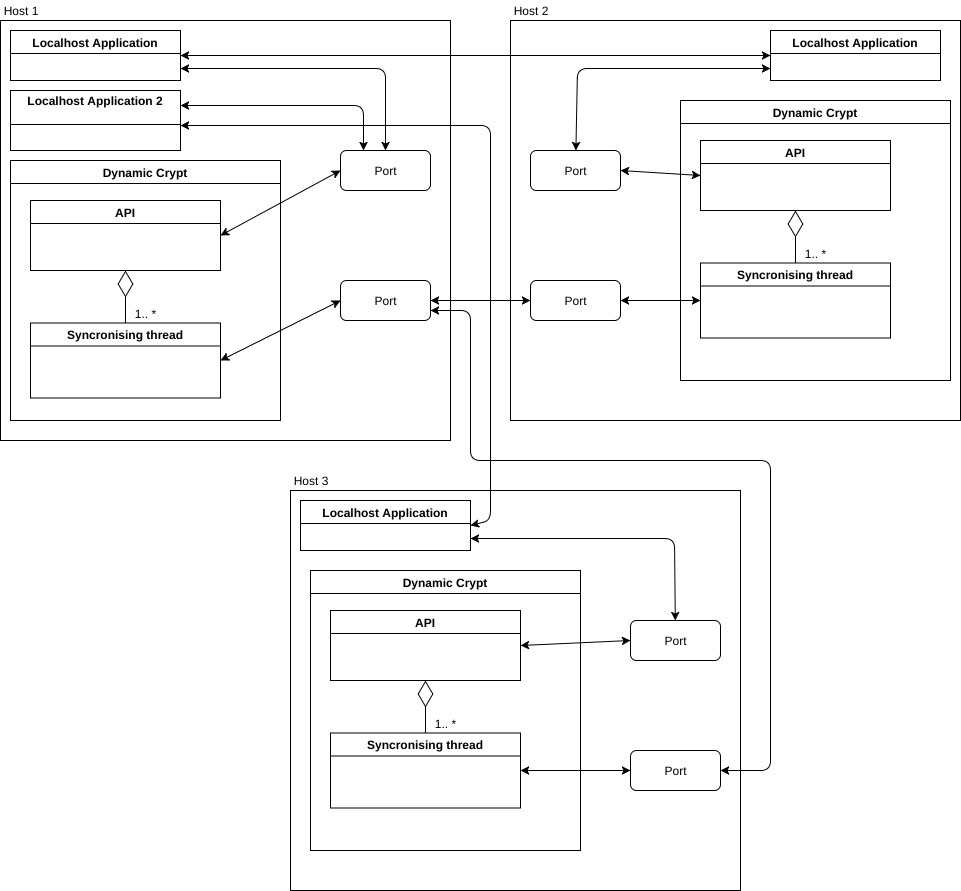
\includegraphics[width=1\textwidth]{Figures/basic-3hosts-2apps.jpg}
  \caption[Host one using Dynamic Crypt System with host two and three with different applications using the API]{Host one using Dynamic Crypt System with host two and three with different applications using the API}
  \label{fig:3hostsbasic2apps}
\end{figure}

\FloatBarrier

The diagram \ref{fig:3hostsbasic2apps} is quite similar to the last example where as in this case there are two local host applications running on Host 1: In this case localhost application 1 is using the dynamic encryption system to send data to Host 2 and localhost application 2 is using the dynamic encryption system to send data to Host 3. They both use the same API and therefore this example is quite similar to the previous one.

Host 1: Localhost application 1 establishes a connection with Host 2: Localhost application using standard methods.
Similarly Host 1: Localhost application 2 establishes a connection with Host 3: Localhost application using standard methods.

Host 1: Localhost application 1 contacts the Host 1: Dynamic Crypt API with an init request. 
Host 1: Localhost application 2 contacts the Host 1: Dynamic Crypt API with an init request. 

Host 1: Dynamic Crypt API takes note of Host 1: Localhost application 1 details such as the applications name or something to distinguish it from Host 1: Localhost application 2, and initialises ten Synchronising threads. The API associates this list of synchronising threads with the application and sends back the details of each thread, the port the threads will use and the IP of Host 1 to Host 1: Localhost application 1 and similar but different values are sent to Host 1: Localhost application 2 as well. 

Host 1: Localhost application 1 forwards this information to Host 2: Localhost application which will know that this is an dynamic synchronisation init request and will forward that information to Host 2: Dynamic Crypt API through the Host 2: Dynamic Crypt API port. 
Host 1: Localhost application 2 forwards this information to Host 3: Localhost application which will know that this is an dynamic synchronisation init request and will forward that information to Host 3: Dynamic Crypt API through the Host 2: Dynamic Crypt API port. 
The Host 2: Dynamic Crypt API and The Host 3: Dynamic Crypt API will initialise ten Synchronising threads and assigns a partner to them which is essentially the partner id of one of the Host 1: Dynamic Crypt threads.

Host 2: Dynamic Crypt threads will send a request to Host 1: Dynamic Crypt threads followed by another request from Host 3: Dynamic Crypt threads to Host 1: Dynamic Crypt threads. The Thread manager will then forward the info to each thread assigning the partners thread id for Host 1 threads. Now synchronisation between threads will occur.

The last three steps are identical as in the first example.



From the three use case examples the API must be able to support:
\begin{itemize}
    \item A single localhost application connecting with another dynamic encryption system.
    \item A single localhost application connecting with multiple other dynamic encryption systems.
    \item Multiple localhost applications connecting with other dynamic encryption systems.
    \item Multiple localhost applications connecting with multiple other dynamic encryption systems per each local host application.
\end{itemize}

\begin{figure}[!h]
  \centering
      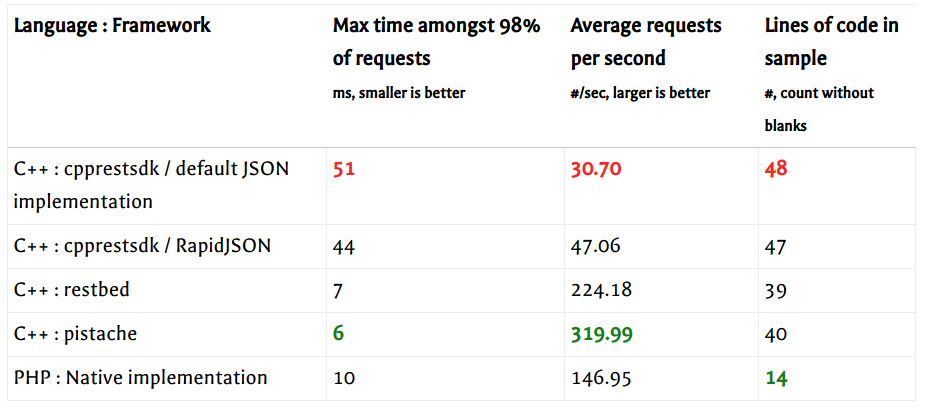
\includegraphics[width=1\textwidth]{Figures/cppframeworks.png}
  \caption[Comparison of different C++ rest frameworks]{Comparison of different C++ rest frameworks\cite{Crestframeworks}}
  \label{fig:Crestframeworks}
\end{figure}

\FloatBarrier

In order to build a proper API I will use a framework as making one from scratch would be too time consuming. There are not many C++ only rest APIs frameworks so the choice was not too difficult. 
Table \ref{fig:Crestframeworks} shows the most popular C++ rest frameworks. Cpprestsdk is made by Microsoft and is generally the most popular one to use. However I have tried installing the library and had issues compiling the examples provided on their GitHub a simple hello world server worked perfectly but the rest API example had issues. This is perhaps for the better that I was unable to get it to work and had to find other frameworks to work with. I stumbled upon the websites that the table is from and the framework Pistache \cite{pistache} seems to be leaps ahead of Cpprestsdk having a low request time of only 6 milliseconds and a large 320 requests per second capability which is what I need for this project and considering that it will take quite a lot of requests to synchronise tree parity machines. Fortunately I was able to install the library correctly and the example rest API code for Pistache compiled and worked correctly.

Therefore I will be using Pistache as the rest API part of this project and the tree parity part of the code also since I wanted my software to utilise two ports.



\begin{figure}[!h]
  \centering
      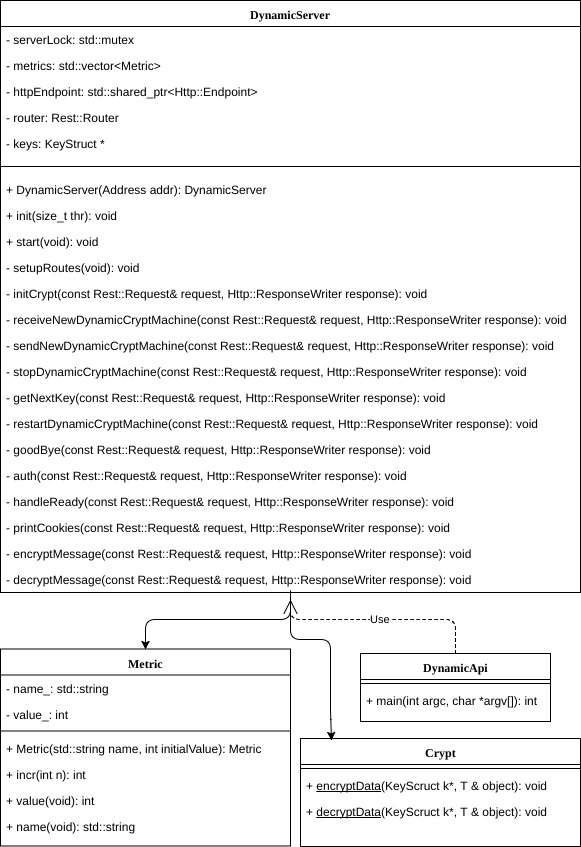
\includegraphics[width=1\textwidth]{Figures/API.jpg}
  \caption[Rest API class diagram]{Rest API class diagram}
  \label{fig:myapi}
\end{figure}

\FloatBarrier

The class diagram \ref{fig:Crestframeworks} demonstrates roughly how the API will look like. The variables at the top of the DynamicServer class are mostly used for the library. serverLock is to prevent issues with threads changing the same variable at the same time. metrics is for measuring various server performances this uses the Metric class defined in the diagram. httpEndpoint is a pointer used by the framework internally. router is used for handling different routes in the setupRoutes function. keys is a struct array that has the generated encryption key from the tree parity machine, the id of the tree parity machine and a status whether it was sent of or not more properties will most likely be added in the implementation phase to this struct.

The functions after setupRoutes are all route handlers that will need to be associated with a route in the setupRoutes function. initCrypt function will tell the tree parity machine handler to setup the tree parity machines. receiveNewDynamicCryptMachine is when a different host setup the tree parity machines and sends you ids and other information to allow for partnering of this hosts tree parity machines. sendNewDynamicCryptMachine is the opposite of the previous this time the api is sending info of its tree parity machines to another host. stopDynamicCryptMachine this is used when the application believes it doesnt need any more new keys for dynamic encryption so the synchronisation will cease to avoid expensive unnecessary operations. getNextKey will send the next if available key to the application. restartDynamicCryptMachine would be typically called after stopDynamicCryptMachine to generate more keys once again. goodBye will be called when the application doesn't need to use the API anymore this will remove any references and any tree parity machines relating to the application. When the application disconnects from the API a similiar set of instructions will also occur. auth is when authorisation will be implemented for increased security. handleReady is more of a test function to determine if server is up and running. printCookies will most likely never be used. The encryptMessage and decryptMessage allow the user to pass in a message to be encrypted. The Crypt class will handle the encryption and decryption of such data. The KeyStruct struct will contain information about which tree parity machine generated the key so there will be no confusion when encrypting and decrypting between multiple hosts.

The Metric class is used for saving different server metrics. A metric has a name, value and increment amount.

Lastly the DynamicApi class holds the main method that initialises the server.






\begin{figure}[!h]
  \centering
      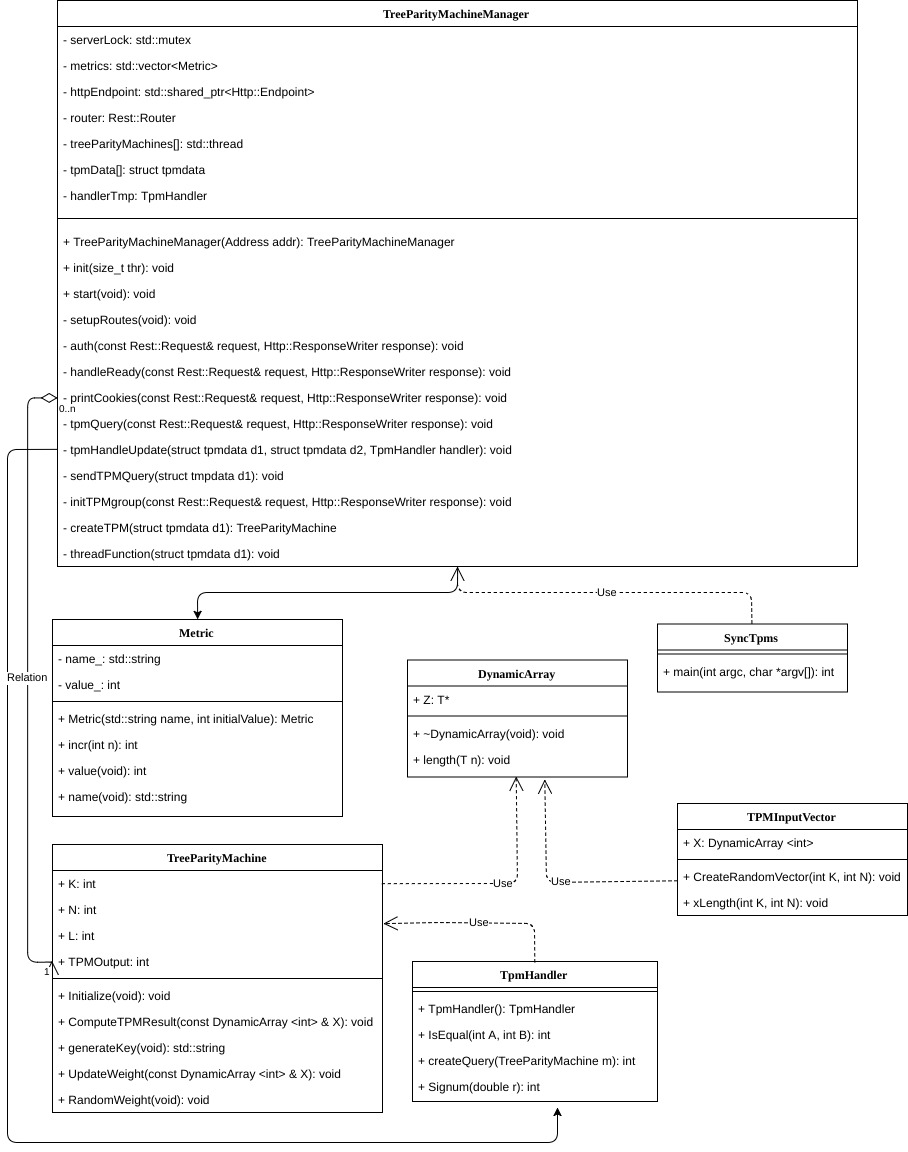
\includegraphics[width=1\textwidth]{Figures/TreeParityMachineManager.jpg}
  \caption[Tree Parity Machine Manager class diagram]{Tree Parity Machine Manager class diagram}
  \label{fig:tpmmanagerClassDiagram}
\end{figure}

\FloatBarrier

This is a class diagram\ref{fig:tpmmanagerClassDiagram} of the second application. There are two applications primarily because it will be easier and less strain on the API server if the synchronisation activities were running on a different server. These servers will communicate with each other via network protocols and or via shared memory which will be discussed later in this section. The TreeParityMachineManager class has similar variables and functions as DynamicServer from the previous diagram because both of them are implementing the Pistache server framework. Therefore I wont mention the variables and functions required for the framework here again. This class may have to implement the main method as it requires multithreading but I will have to do some tests before I can finilise my answer. 

The threads will be held in an array called treeParityMachines and each thread will execute the function threadFunction which will be used to process the tree parity machines. a struct tpmdata will be passed in to this function, this struct will hold the information and pointers for each tree parity machine and information of the thread that is executing that tree parity machine. The tpmQuery and sendTPMQuery functions will send and receive queries from different hosts to syncronise the tree parity machine. tpmHandleUpdate function is called inside the tpmQuery and sendTPMQuery functions and will update the tree parity machine weights if needed accordingly. initTPMgroup function will create a group of partner tree parity machines for each host that connects with the help of the createTPM function which takes a tmpdata struct and updates it when the tree parity machine is created.

The TreeParityMachine class is the actual tree parity machine itself. K,N,L are tree parity machine parameters these will be discussed later in this section. The TPMOutput is the output of the machine after a query is received. This class has some basic functions required for the tree parity machine to operate. Initialize will initialise the tree parity machine with random weights. ComputeTPMResult will update the TPMOutput variable after processing a query. generateKey willl generate a key based on the tree parity machines weights. UpdateWeight updates the weights if needed. RandomWeight sets the tree parity machines weights to random weights.

The TpmHandler class help out in synchronising the partner tree parity machine with the one locally stored on this host. IsEqual checks if the output bits of both syncronising tree parity machines is equal and therefore other functions can proceed to update weights or not. createQuery creates a query based on the tree parity machines weights. Signum is used for calculations. 

The DynamicArray is used for an adaptable array needed for the TreeParityMachine class. The TPMInputVector class is a helper for creating a vector that is also used by the TreeParityMachine class.

And lastly the SyncTpms holds a main method which might be removed in the implementation phase as there could be issues with threads I will have to experiment to determine this outcome.



\begin{figure}[!h]
  \centering
      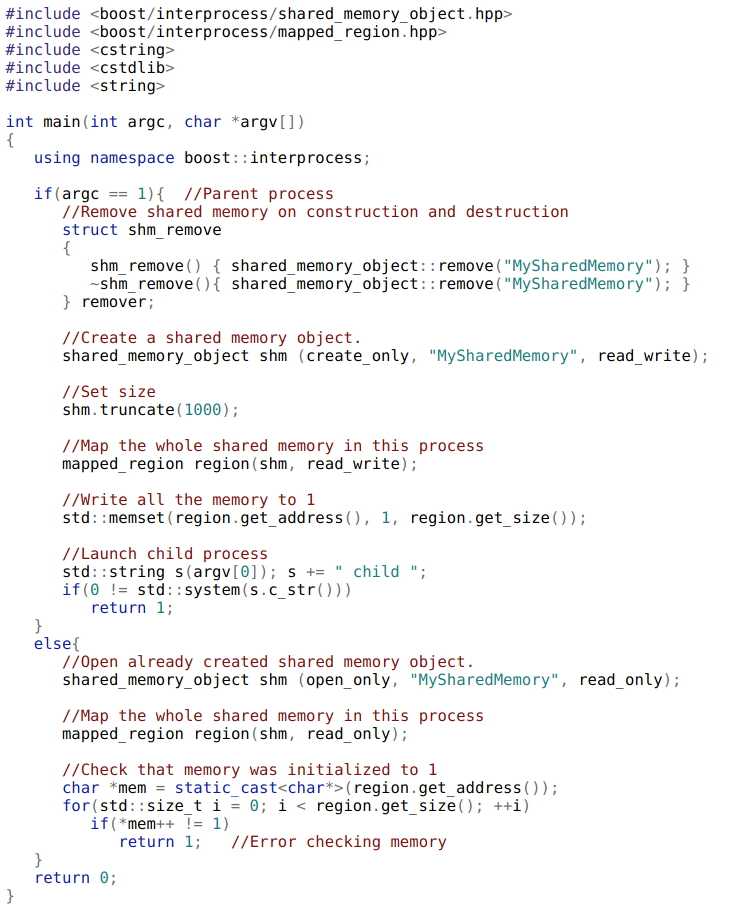
\includegraphics[width=1\textwidth]{Figures/boost.png}
  \caption[shared memory with boost]{shared memory with boost\cite{boost}}
  \label{fig:boostEzcode}
\end{figure}

\FloatBarrier

The two applications that I am building are executed on the same host therefore it would be in my best interest to share a chunk of memory between them not only will this increase performance as accessing shared memory is much faster than using networking protocols. Using shared memory will also alleviate some of the stress that would be induced on the servers as they would need to communicate between themselves. To achieve this in a timely manner i will use the help of the boost \cite{boost} library which includes functions for shared memory management.

The source code for a simple implementation can be found on the boost website which is included in figure \ref{fig:boostEzcode}. One application would have to initiate a memory region with 
\begin{lstlisting}[language=C] 
mathshared_memory_object shm (create_only, "MySharedMemory", read_write); 
\end{lstlisting}
The other server can then open this shared memory using the following
\begin{lstlisting}[language=C] 
shared_memory_object shm (open_only, "MySharedMemory", read_only);
\end{lstlisting}
Before using the shared memory it must be mapped to the process therefore both processes will need the following
\begin{lstlisting}[language=C] 
mapped_region region(shm, read_only);
\end{lstlisting}

Lastly to make this project easily adaptable I will be making a NodeJS module or specifically middleware compatible with ExpressJS \cite{ExpressJS}. Middleware in NodeJS is functions that take the request or response and process it in some way or form and return or send the modified request or response to the user see figure \ref{fig:middlewarebasic}. My project is definitely usable without this module however this will simplify things even further for people who wish to use this project with NodeJS. 

\begin{figure}[!h]
  \centering
      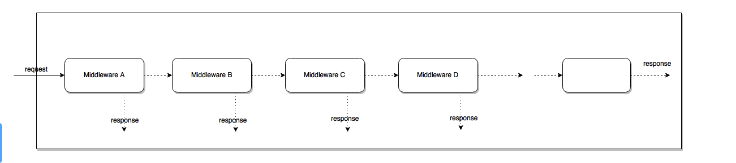
\includegraphics[width=1\textwidth]{Figures/middleware.png}
  \caption[middleware in express]{middleware in express \cite{middleware}}
  \label{fig:middlewarebasic}
\end{figure}

\FloatBarrier

This middleware will be mostly interacting with the DynamicServer API and will use promises that will return various information when said information is acquired, it might take a while for the initial key to arrive so I believe promises would be the best way to go. 

\begin{figure}[!h]
  \centering
      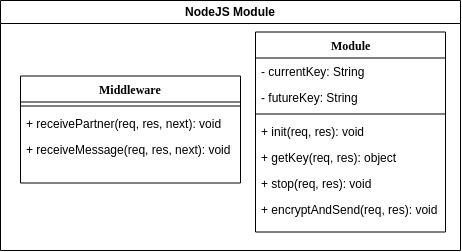
\includegraphics[width=0.7\textwidth]{Figures/NodeJsModule.jpg}
  \caption[NodeJS Module diagram]{NodeJs Module diagram}
  \label{fig:mynodemoduleclass}
\end{figure}

\FloatBarrier

The diagram \ref{fig:mynodemoduleclass} is a bare bones representation of what the NodeJS module will look like. I will be doing this part last during the implementation phase so a lot will change by then and therefore this isn't described in too much detail. Since JavaScript can't really be represented in a class diagram I have split the methods onto middleware functionality and everything that is not middleware is represented in the module class.

The methods in the middleware are as follows:
receivePartner this will perform actions if the request is part of the dynamic encryption and specifically the one that asks the server to use dynamic encryption if the request is anything else the middleware will just call next() and the next middleware in line will perform functions. This function will call the init route in the API with the information of the partner and perhaps more functionality will be required during the implementation phase. This functionality needs to be implemented as middleware since the other host can request to use dynamic encryption with this host at any time.
receiveMessage will detect if the response is using dynamic encryption and will decrypt that message and update the response object with the decrypted message.

The methods in the module are as follows:
init will send a request to the init route in the API like the receivePartner method but without the partner information.
getKey will request a new key from the API.
stop will stop all syncronising tree parity machines for when dynamic encryption is not needed anymore. It is possible to call init once more to continue syncronisaton. 
encryptAndSend encrypts a passed in message and sends it to the other host.
There are two variables in the module currentKey and futureKey. When you call getKey there may be encrypted messages that arrive at a later time and therefore will use currentKey for decryption and newer messages will use futureKey.   


























\section{Risk Assessment}
%Identify any potential risk precluding you from successfully complete your project. This section is really important and often neglected by students resulting in fatal risks occurring in some projects. Make sure to give this section the time it requires. Classify the risk according to their importance, possibility of arising and enumerate the decisions you can make to anticipate them or mitigate them (in case they finally arise). Table \ref{tab:ProjRisks} may help with this classification. This section should include your mitigation approach for any critical risks.

%\begin{table}[h]
%\centering
%\scriptsize
%\caption{Initial risk matrix}
%\begin{tabular}{|p{2cm}|p{2cm}|p{2cm}| p{2cm} |p{2cm}| p{2cm}|}
%\hline \bf Frequency/ Consequence & \bf 1-Rare & \bf 2-Remote & \bf 3-Occasional & \bf 4-Probable & \bf 5-Frequent\\ [10pt]

%\hline \bf 4-Fatal & \cellcolor{yellow!50} & \cellcolor{red!50} & \cellcolor{red!50} & \cellcolor{red!50} &\cellcolor{red!50} \\ [10pt]

%\hline \bf 3-Critical &\cellcolor{green!50} & \cellcolor{yellow!50} & \cellcolor{yellow!50} & \cellcolor{red!50} &\cellcolor{red!50} \\ [10pt]

%\hline \bf 2-Major & \cellcolor{green!50} & \cellcolor{green!50} & \cellcolor{yellow!50} &\cellcolor{yellow!50} &\cellcolor{red!50} \\ [10pt]

%\hline \bf 1-Minor & \cellcolor{green!50} & \cellcolor{green!50} & \cellcolor{green!50} &\cellcolor{yellow!50} &\cellcolor{yellow!50} \\ [10pt]
%\hline
%\end{tabular} \\
%\label{tab:ProjRisks}
%\end{table}
Creating a reasonably complex project leads to a possibility of risks that may potentially cause my project to fail. This involves risks such as technical issues, implementation issues and design issues. 

The amount of data transferred between each tree parity machine might overwhelm the servers due to many tree parity machines synchronising at once. This can lead to very slow operation or servers crashing therefore I may have to run multiple instances of the servers or reduce the number of tree parity machines.

This project uses a lot of specific algorithms that are projected through mathematical formulas. Failure to understand or implement these formulas into code can cause a delay or failure to complete some functionality.

The framework that I'm planning on using for the rest APIs might not be suitable for the task. This is unlikely to happen as I have researched the most responsive rest frameworks. Pistache seems to have the highest request per second processing time.

This project relies on having a stable network to send data to and from different hosts. A network failure would cause the synchronisation process to cease. Or a congested network will slow down the synchronisation process to an unusable state where it would take a very long time to synchronise due to a plethora of lost packages.

A number of C++ libraries are used for this project as well as some NodeJS libraries that could potentially be used for the NodeJS module. The availability of these libraries could cease or they could become closed source will cause issues in finding alternatives. 

%C++ and JavaScript in particular the NodeJS library are the main languages used in this project if they become unavailable due to the internet lines getting eaten by zombies due to the inevitable zombie Apocalypse I will need to develop my own programming languages using sticks and stones since zues will come down to earth and siphen all of the electricity all while defending myself against the endless hords of the undead and crazy ass pickacho's infected with rabies.

C++ and JavaScript in particular the NodeJS library are the main languages used in this project if they become unavailable I will have to research and implement the project in other languages.

Due to this project being self managed poor planning such as task estimation time or spending too long on a single task may cause the project to be not finished at the deadline set.

This project is built using primarily one device which can lead to laziness with backups. The project should be backed up to an external hard drive or because I am using git for version management I will be occasionally pushing it to GitHub.


\section{Methodology}
%Describe your personal approach on how to tackle the different parts of this project, including:
%\begin{itemize}
%    \item How to tackle the needed research to fulfill the background chapter. 
%    \item How to set up your Computer Science skills to the project needs (e.g., describe your plan to learn any new technology involved on the project that you are not familiar with). 
%    \item What core project managing approach will you follow (e.g., Waterfall, Scrum, etc).
%\end{itemize}


I employed a various range of techniques while finalising the background chapter of this paper. I initially researched any reference or any details about dynamic encryption and discovered that it is a mildly discussed topic. A closed source product explained briefly that in order to achieve dynamic encryption they use wrappers. I didn't find wrappers very interesting. And because wrappers at the time of my research were the only method of achieving dynamic encryption publicly available I decided to look at the problem from a different perspective.

In order to achieve dynamic encryption the key must essentially be changed this can be done many ways by sending the key over the network however my goal was to not send the key over the open network, at least not directly. 

I researched topics about key generation and other unconventional ways of sharing keys. 
I came across neural network synchronisation which can be used to generate a key without directly sending sensitive information over the network. 

The only information about this topic I could find was in research papers, luckily there was a good number of relevant papers with a reasonable variety of information available. All of these were more or less proof of concept as there were no products or examples based of these. After reading and understanding the similarities between these papers I was able to commence chapter 2. 

While constructing chapter two I outlined what is needed for a tree parity machine to operate and the differences between the possible tree parity machines such as different learning algorithms and the benefit of using queries instead of random inputs all while referencing the resources I had available before hand and using relevant points and diagrams from those resources.




Most of the computer science skills required for this project I already posses like building a NodeJS module. However there are many aspects of the project which are new to me. Starting of with the main language C++, which I do not know as well as C however I have used C++ many times in the past as I find multithreading and sleep style functions to be more diverse in C++ as well as the fact that C++ is object orientated making C more difficult to use for larger projects. My C++ skills will need to be expanded a little bit more to complete this project. I have never wrote a rest API server using anything other than NodeJS therefore writing it in C++ is new to me, however I have researched a number of C++ rest frameworks and found Pistache to be similar enough to what I recall from NodeJS and was able to reasonably understand and execute the example server code provided on the Pistache GitHub. I will have to experiment with incorporating custom multithreading functions with Pistache as that might cause issues with multiple clients connected.
I will also attempt to implement memory sharing between two applications to minimise the stress on the network part of the programs. I have never used shared memory in the past however the library boost provides methods that can be used to allocate a block of memory to be shared amongst applications. I am able to use and understand the basic example however the memory there is constantly the same size which will not be the case in this project so I will need to experiment with this.






For this project I will agile mythology in particular a sprint based one, where I will undergo a two week sprint followed by a retrospective and planning for the next sprint. I have chosen to follow this technique as that is what was used during my work placement in a well known company. 

It is also very unlikely that a project can be fully created just from class diagrams, ideas and functionality all at the very beginning. Issues and further functionality may have to be resolved and introduced in order to provide a working product, there is no way to predict the exact way to develop software without actually making a basic version and expanding on it until all the features required are implemented and fully working. 

This technique is commonly used for projects will multiple people however there is no harm in following this even if the project only consists of one member. 
I believe it is important to follow industry standard methods as much as possible since these methods are developed and used by the top companies on earth therefore using these methods must be the best way to accomplish projects as of writing this paper.


\section{Implementation Plan Schedule}
%Come up with a schedule for the remaining time (including second semester), so as to describe how do you envision to achieve the implementation of your project by the end of semester 2. This plan SHOULD be ambitious but MUST be realistic and SHOULD be informed by early prototyping and MUST be discussed with your term 1 supervisor.
I will be using agile methodology in particular two week sprints followed by sprint retrospect and sprint planning after each sprint is completed. Therefore it is difficult to put a schedule as the next sprint is usually planned after and typically based on the outcome of the sprint before hand. 
Bellow is a rough description for each sprint if everything goes according to plan.


\begin{table}[h]
\centering
\caption{Sprint Plan}
\begin{tabular}{|p{1cm}|p{12cm}|}
\hline Sprint & Tasks \\ [14pt]

\hline 1 & Expand prototype to work with two process instances instead of just in the same process. Can use normal files to communicate. \\ [12pt]

\hline 2 & Implement the use of queries instead of random inputs. \\ [12pt]

\hline 3 & Create basic rest server and experiment with multithreading and multiple clients. \\ [12pt]

\hline 4 & Extend functionality of server to mock synchronisation between identical server on a different hosts. e.g. send incremental data to and from each host.\\ [12pt]

\hline 5 & Replace mock with a real tree parity machine. \\ [12pt]

\hline 6 & Add support for multiple tree parity machines. This will need to be stress tested and load tested to ensure that the server lasts under heavy conditions. \\ [12pt]

\hline 7 & Develop the API server for communicating with local host servers. \\ [12pt]

\hline 8 & Develop NodeJS module. \\ [12pt]

\hline 9 & Implement and allow multiple instances to run for performance and stability increase. \\ [12pt]

\hline 10 & Thoroughly test system including NodeJS module and fix any remaining bugs. \\ [12pt]

\hline
\end{tabular} \\
\label{tab:ProjRisks}
\end{table}

\FloatBarrier



\section{Evaluation}
%Come up with an evaluation plan that allows you to measure how much have you actually achieved the goals of your project. This again is a section that is often neglected where students loose marks. How do you plan to measure the output of your project? A binary it works/does not work is insufficient. You need to be able to quantify the success against both the functional requirements and the initial idea. These are not the same as you may meet all function requirements outlined but not solve the overall problem because you have failed to revisit these and update them with new information which you learn as you are developing the project.
The evaluation of this project can be conceived by examining if the functional and non functional requirements are met. The goals aimed to be achieved by this project will also be compared with the final project. 

The final project should be able to successfully synchronise with another instance preferably running on a different host for realism and be able to synchronise using multiple tree parity machines.

The project should not be vulnerable to tree parity machine attacks, this is unlikely as using queries will negate any possible attack methods known.

The communication between the tree parity machine manager and API should be secure and robust. 

An encrypted message send from host 1 should be successfully decrypted after it arrives to host 2.

The NodeJS module should be easy to use and can be implemented in any NodeJS project provided ExpressJS is used.

\section{Prototype}
%Although you do not have a fully functional project yet, you should show wireframes, snapshots or representation on how do you envision your project to look once the implementation phase has been completed. The nature of this section will vary significantly from project to project and can include anything from code snippets to snapshots of service deployments. Any prototyping you have done during the term should be summarized here that has not been captured in earlier sections. For example if you are planning to host your project using AWS in an EC2 instance you should have at least created a "hello world" setup to determine the basics, this probably should have been discussed in section \ref{sec:Arch}.
The prototype can be found on my GitHub here \cite{prototype-github}. This prototype borrows pieces of code from here \cite{SagunmsNeuroCrypto} and demonstrates a very simple synchronisation method between two tree parity machines. The Prototype consists of two tree parity machines that synchronise with each other using random input vectors. The finial version of the tree parity machines will use queries instead of random input vectors this will result in faster synchronisation time and tree parity machine attacks will not be possible when using queries making it secure.
The prototype has both tree parity machines running in the same main function so there is no networking involved thus the two tree parity machines can be accessed easily and freely.   
\begin{figure}[!h]
  \centering
      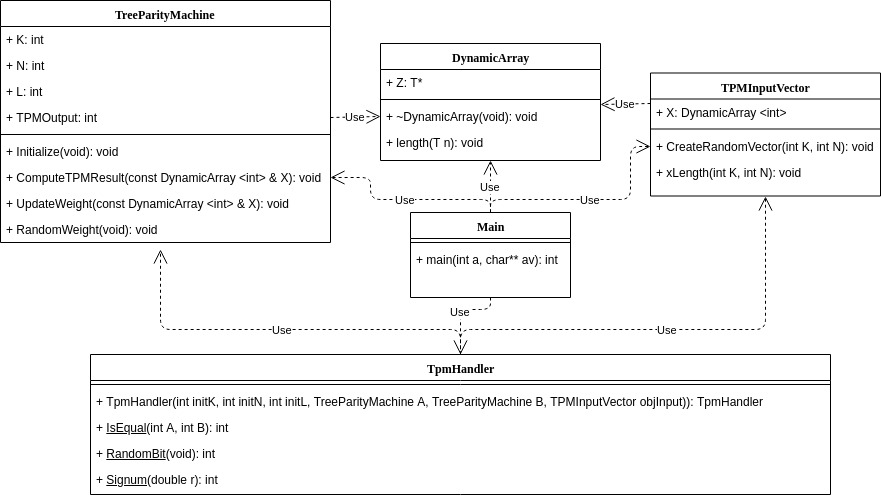
\includegraphics[width=1\textwidth]{Figures/TreeParityMachine.jpg}
  \caption[Prototype class diagram]{Prototype class diagram}
  \label{fig:prototype}
\end{figure}

\FloatBarrier

This is a class diagram of the prototype \ref{fig:prototype}. Since the two tree parity machines synchronise with each other in the same process the diagram is quite small.

\begin{figure}[!h]
  \centering
      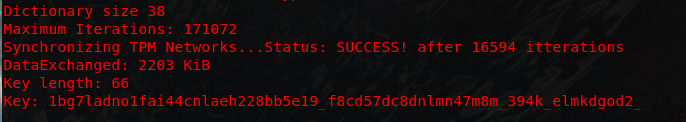
\includegraphics[width=1\textwidth]{Figures/proto2.png}
  \caption[Prototype in action]{Prototype in action}
  \label{fig:prototype2}
\end{figure}
\FloatBarrier

\FloatBarrier
Figure \ref{fig:prototype2} shows a successful synchronisation between the two tree parity machines.
This run uses the following tree parity machine parameters 12 input neutrons, 11 hidden neutrons and a weight range of 6 meaning the possible value for each weight element is from -6 to 6.  
The Dictionary size refers to an array from which different elements will be picked to build the encryption key seen on the last line.

\begin{figure}[!h]
  \centering
      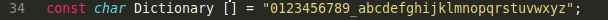
\includegraphics[width=1\textwidth]{Figures/proto4.png}
  \caption[Dictionary used]{Dictionary used}
  \label{fig:prototype4}
\end{figure}
\FloatBarrier
The code snippet \ref{fig:prototype4} contains all the possible characters possible that will make up the key. 

Maximum Iterations is the maximum times the tree parity machines will receive input in order to synchronise. This is used just in case something goes wrong the tree parity machines will not be trying to synchronise forever. The Maximum Iterations is calculated based on the input neutrons, hidden neutrons and the range of weight values. The Maximum Iterations is calculated in this case to be 171,072 which is quite a lot however the tree parity machines manage to synchronise way before that number is reached. In this run the tree parity machines synchronised successfully after 16,594 iterations. 
DataExchanged is an estimation of the amount of data required to synchronise the two tree parity machines. This is mostly affected by the number of iterations taken to synchronise the more iterations the higher the data. 
Using the above stated tree parity machine parameters a key of length 66 is produced, increasing and decreasing the tree parity machine parameters will have an impact on the key size.


\begin{figure}[!h]
  \centering
      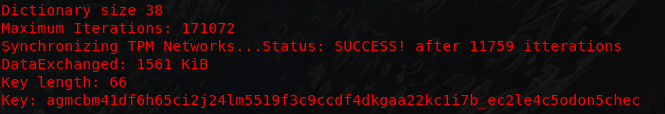
\includegraphics[width=1\textwidth]{Figures/proto3.png}
  \caption[Prototype in action]{Prototype in action}
  \label{fig:prototype3}
\end{figure}

\FloatBarrier
Figure \ref{fig:prototype3} shows another successful synchronisation between the two tree parity machines using the same tree parity machine parameters as the previous example. The key in this case is obviously different and so is the number of iterations required to synchronise. This also means that the amount if estimated data is less in this case it is 642 KiB less.

By changing the tree parity machine parameter variables to lower values of 8 for the hidden neutrons, 10 input neutrons and a weight range of 4 the encryption key is now 20 characters long. Figures \ref{fig:prototype5} and \ref{fig:prototype6} are executed using this configuration.

\begin{figure}[!h]
  \centering
      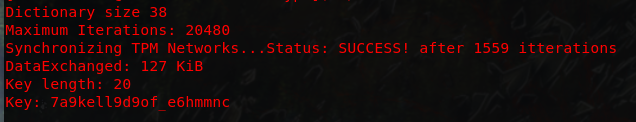
\includegraphics[width=1\textwidth]{Figures/proto5.png}
  \caption[Prototype in action with a key size of 20]{Prototype in action with a key size of 20}
  \label{fig:prototype5}
\end{figure}
\FloatBarrier
Because the number of neutrons is reduced so is the number of weight and therefore the number of iterations required for synchronisation is reduced to only 1,559 in figure \ref{fig:prototype5} and 3,661 in figure \ref{fig:prototype6} which is considerably smaller than 11,759 and 16,594 seen before. 



\begin{figure}[!h]
  \centering
      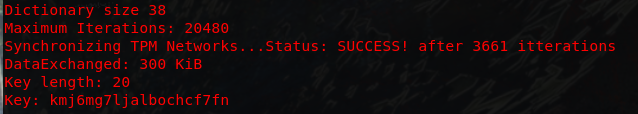
\includegraphics[width=1\textwidth]{Figures/proto6.png}
  \caption[Prototype in action with a key size of 20]{Prototype in action with a key size of 20}
  \label{fig:prototype6}
\end{figure}
\FloatBarrier

The data exchanged is also significantly reduced with the fewer number of iterations with only 127 KiB in \ref{fig:prototype5} and 300 KiB in figure \ref{fig:prototype6} compared to 2,203 KiB and 1561 KiB in the previous two examples.

In order for synchronisation to occur the weights of both tree parity machines must be identical since the generated key is based on them. The weights are essentially an Array or specifically they are an DynamicArray object and thus can be represented.

\begin{figure}[!h]
  \centering
      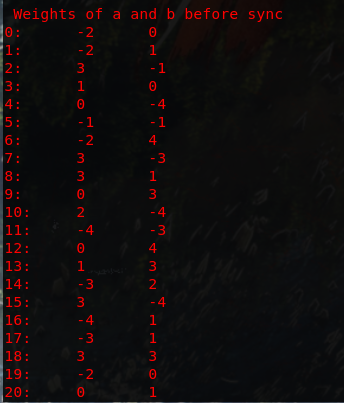
\includegraphics[width=0.6\textwidth]{Figures/proto7.png}
  \caption[Weights of A and B before synchronisation]{Weights of A and B before synchronisation}
  \label{fig:prototype7}
\end{figure}
\FloatBarrier
The figure \ref{fig:prototype7} is the representation of the fist 21 weight values, there is a total of 80 weight values because this run is using 8 hidden neutrons and 10 input neutrons and therefore the size of the list of weight values is 8 * 10. The first column just shows the number in the list for which this weight is associated with. The second column is the weights of the tree parity machine A and the third column is the weights of the tree parity machine B. 
These weights are displayed before the synchronisation process begins and as you can see they are nothing alike. Note that the maximum and minimum values you can see is -4 to 4 this is because the weight range for this run is set to 4.



\begin{figure}[!h]
  \centering
      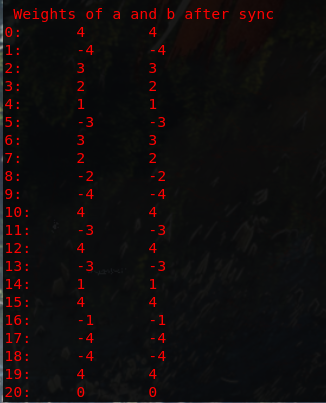
\includegraphics[width=0.6\textwidth]{Figures/proto8.png}
  \caption[Weights of A and B after synchronisation]{Weights of A and B after synchronisation}
  \label{fig:prototype8}
\end{figure}
\FloatBarrier

The figure \ref{fig:prototype8} is taken from the same run but the weights are displayed after the synchronisation process and as you can see the weights of both of the tree parity machines are now identical therefore they are able to produce the same key.

\begin{figure}[!h]
  \centering
      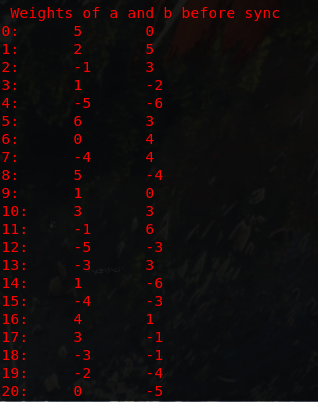
\includegraphics[width=0.6\textwidth]{Figures/proto9.png}
  \caption[Weights of A and B before synchronisation with an increased range]{Weights of A and B before synchronisation with an increased range}
  \label{fig:prototype9}
\end{figure}
\FloatBarrier
The figure \ref{fig:prototype9} is displaying the weights of both tree parity machines before synchronisation just like before except this time the weight range is increased to 6 that's is why the minimum and maximum values you can see this time is -6 to 6. Again the weights are completely different from one another as they are initialised randomly at the beginning. In the prototype time is used to seed the random generator this will not be acceptable for the final project as time can be easily guessed. 


\begin{figure}[!h]
  \centering
      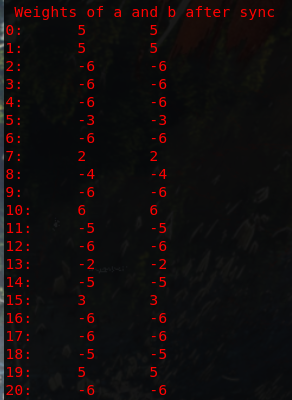
\includegraphics[width=0.6\textwidth]{Figures/proto10.png}
  \caption[Weights of A and B after synchronisation with an increased range]{Weights of A and B after synchronisation with an increased range}
  \label{fig:prototype10}
\end{figure}
\FloatBarrier
The figure \ref{fig:prototype10} is the weights of the same tree parity machines as in figure \ref{fig:prototype9} but after synchronisation and as you can see the weights are now identical. 
The reason one might choose to increase the weight range is because these weight are used in calculations and give a little bit more diversity. 
Increasing the weight range can also increase the length of the encryption key. Figure \ref{fig:prototype7} uses the same parameters as \ref{fig:prototype10} but with a weight range of 4 instead of 6. The key length of \ref{fig:prototype7} is 20 and the key length of \ref{fig:prototype10} is 40.
In my testing I found that there isn't really any benefit in increasing the weight range past 6 as anything above 6 doesn't increase the key length by much and increases the number of iterations by a good bit. I have found that it is better to increase the number of hidden neutrons if you need a larger key length followed by the number of input neutrons and just leave the weight range at 6.


%most of the work like the iterations was done in the main function so I will go through the important bits before demonstrating an example of it running.

%\begin{figure}[!h]
%  \centering
%      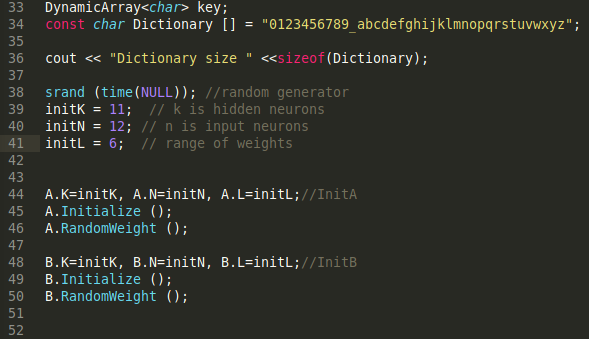
\includegraphics[width=1\textwidth]{Figures/proto1.png}
%%  \caption[Prototype code section]{Prototype code section}
%  \label{fig:prototype1}
%\end{figure}

%\FloatBarrier
%The figure \ref{fig:prototype} is a snippet of code 